% !TeX root = D4.1a_User_Manual.tex
Overture implements export of both tool-wrapper as well as standalone FMUs.
%
It also has the ability to import a \texttt{model\-Description.\allowbreak{}xml} file in order to facilitate creating an FMI-compliant model from scratch.
%
A typical workflow in creating a new FMI-compliant VDM-RT model starts with the import of a \texttt{model\-Description.\allowbreak{}xml} file created using Modelio.
%
This results in a minimal project that can be exported as an FMU.
%
The desired model is then developed in this context.
%
This section discusses the complete workflow.
%
%
%
\subsubsection{Installing the FMI import/export plugin for Overture}
In order to use the FMI integration in Overture it is necessary to install a plugin.
Below is a guide to install the plugin:
\begin{enumerate}
	\item Open Overture.
	\item Select \textit{Help} -> \textit{Install New Software}.
	\item Click \textit{Add..}.
	\item In the \textit{Name:} field write \textit{Overture FMU}.
	\item In the \textit{Location:} field there are two options:
		\begin{description}
			\item[INTO-CPS Application:] Download the \textit{Overture FMU Import / Exporter - Overture FMI Support} using the Download Manager mentioned in Section \ref{sub:other-features}. Locate the file using the \textit{Archive...} button next to the \textit{Location:} field.
			\item[Update site:] Enter the following URL in the \textit{Location:} field: \\ \textit{http://overture.au.dk/into-cps/vdm-tool-wrapper/master/latest}.
		\end{description}
	\item Check the box next to \textit{Overture FMI Integration} as shown in Figure \ref{fig:importFMIoverture}.
	\item Click \textit{Next} or \textit{Finish} to accept and install.
\end{enumerate}
\begin{figure}[ht]
	\centering
	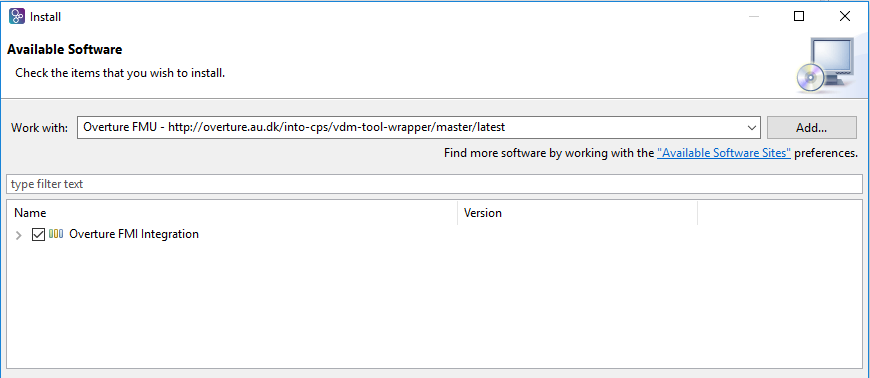
\includegraphics[width=5in]{figures/installOvertureFmiIntegration.png}
	\caption{Installing Overture FMI Integration.}
	\label{fig:importFMIoverture}
\end{figure}
%
%
%
\subsubsection{Import of \texttt{model\-Description.\allowbreak{}xml} File}
A \texttt{model\-Description.\allowbreak{}xml} file is easily imported into an existing, typically blank, VDM-RT project from the project explorer context menu as shown in Figure \ref{fig:moddescimportoverture}.
%
%
%
\begin{figure}[ht]
\centering
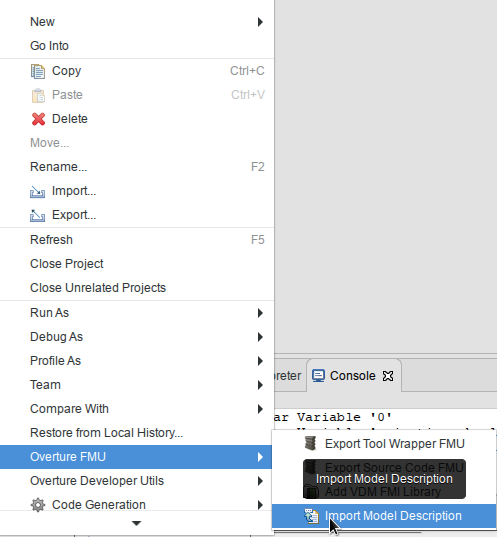
\includegraphics[width=3.7in]{figures/modelDescImportOverture.png}
\caption{Importing a \texttt{model\-Description.\allowbreak{}xml} file.}
\label{fig:moddescimportoverture}
\end{figure}
%
%
%
This results in the project being populated with the classes necessary for FMU export:
%
%
%
\begin{itemize}
\item  A VDM-RT \texttt{system} class named ``System'' containing the system definition.  The corresponding ``System'' class for the water tank controller FMU is shown in Listing \ref{lst:wtSystem}.
%
\item  A standard VDM-RT class named ``World''.  This class is conventional and only provides an entry point into the model.  The corresponding ``World'' class for the water tank controller FMU is shown in Listing \ref{lst:wtWorld}.
%
\item  A standard VDM-RT class named ``HardwareInterface''.  This class contains the definition of the input and output ports of the FMU.  Its structure is enforced, and a self-documenting annotation scheme\footnote{The annotation scheme is documented on the INTO-CPS website \url{into-cps-association.github.io} under ``\textit{Constituent Model Development} $\rightarrow$ \textit{Overture} $\rightarrow$ \textit{FMU Import/Export}.} is used such that the ``HardwareInterface'' class may be hand-written.  The corresponding ``HardwareInterface'' class for the water tank controller FMU is shown in Listing \ref{lst:wtHWInterface}.
%
\item  The library file \texttt{Fmi.vdmrt} which defines the hardware interface port types used in ``HardwareInterface''.
\end{itemize}
%
%
%
\begin{figure}[ht]
\begin{vdmrt}
system System

instance variables

-- Hardware interface variable required by FMU Import/Export
public static hwi: HardwareInterface := new HardwareInterface();
    

instance variables

  public levelSensor : LevelSensor;
  public valveActuator : ValveActuator;
  public static controller : [Controller] := nil;

	cpu1 : CPU := new CPU(<FP>, 20);
operations

public System : () ==> System
System () == 
(
	levelSensor := new LevelSensor(hwi.level);
	valveActuator :=  new ValveActuator(hwi.valveState); 
	
	controller := new Controller(levelSensor, valveActuator);

	cpu1.deploy(controller,"Controller");
);

end System
\end{vdmrt}
\caption{``System'' class for water tank controller.}
\label{lst:wtSystem}
\end{figure}
%
%
%
\begin{figure}[ht]
\begin{vdmrt}
class World

operations

public run : () ==> ()
run() ==
 (start(System`controller);
  block();
 );

private block : () ==>()
block() ==
  skip;

sync

  per block => false;

end World
\end{vdmrt}
\caption{``World'' class for water tank controller.}
\label{lst:wtWorld}
\end{figure}
%
%
%
\begin{figure}[ht]
\begin{vdmrt}
class HardwareInterface

values
	-- @ interface: type = parameter, name="minlevel";
	public minlevel : RealPort = new RealPort(1.0);
	-- @ interface: type = parameter, name="maxlevel";
	public maxlevel : RealPort = new RealPort(2.0);

instance variables
	-- @ interface: type = input, name="level";
	public level : RealPort := new RealPort(0.0);

instance variables
	-- @ interface: type = output, name="valve";
	public valveState : BoolPort := new BoolPort(false);

end HardwareInterface
\end{vdmrt}
\caption{``HardwareInterface'' class for water tank controller.}
\label{lst:wtHWInterface}
\end{figure}
\clearpage
%
%
%
The port structure used in the ``HardwareInterface'' class is a simple inheritance structure, with a top-level generic ``Port'', subclassed by ports for specific values:  booleans, reals, integers and strings.
%
The hierarchy is shown in Listing \ref{lst:fmivdmrtFile}.
%
When a model is developed without the benefit of an existing \texttt{model\-Description.\allowbreak{}xml} file, this library file can be added to the project from the project context menu, also under the category ``Overture FMU''.
%
%
%
\begin{figure}[ht]
\begin{vdmrt}
class Port

types
	public String = seq of char;
	public FmiPortType = bool | real | int | String;
 
operations

	public setValue : FmiPortType ==> ()
	setValue(v) == is subclass responsibility;

	public getValue : () ==> FmiPortType
	getValue() == is subclass responsibility;
			
end Port

class IntPort is subclass of Port

instance variables
	value: int:=0;

operations
	public IntPort: int ==> IntPort
	IntPort(v)==setValue(v);

	public setValue : int ==> ()
	setValue(v) ==value :=v;

	public getValue : () ==> int
	getValue() == return value;

end IntPort

class BoolPort is subclass of Port

instance variables
	...
\end{vdmrt}
\caption{Excerpt of ``\texttt{Fmi.vdmrt}'' library file defining FMI interface port hierarchy.}
\label{lst:fmivdmrtFile}
\end{figure}
%
%
%

With all the necessary FMU scaffolding in place, the VDM-RT model can be developed as usual.
%
%
%
\subsubsection{Tool-Wrapper FMU Export}
Models exported as tool-wrapper FMUs require the Overture tool to simulate.
%
Export is implemented such that the VDM interpreter and its FMI interface are included in the exported FMU.
%
Overture tool-wrapper FMUs currently support Win32, Win64, Linux64, Darwin64 and require Java 1.7 to be installed and available in the PATH environment variable.

A tool-wrapper FMU is easily exported from the project context menu as shown in Figure \ref{fig:toolwrapperexportoverture}.
%
The FMU will be placed in the \texttt{generated} folder.
%
%
%
\begin{figure}[ht]
\centering
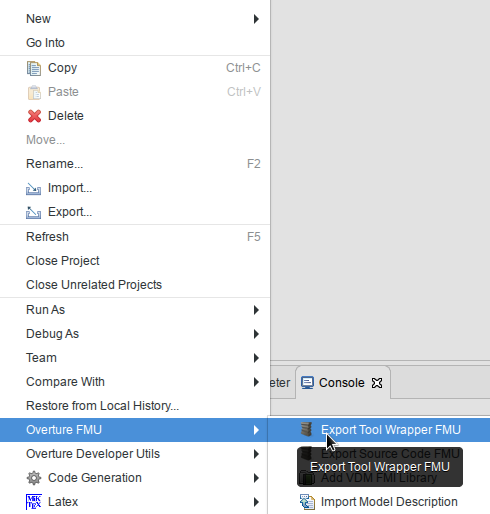
\includegraphics[width=3.5in]{figures/toolWrapperExportOverture.png}
\caption{Exporting a tool-wrapper FMU.}
\label{fig:toolwrapperexportoverture}
\end{figure}
\clearpage
%
%
%
\subsubsection{Standalone FMU Export}
In contrast to tool-wrapper FMUs, models exported as standalone FMUs do not require Overture in order to simulate.
%
Instead, they are first passed through Overture's C code generator such that a standalone implementation of the model is first obtained.
%
Once compiled, this executable model then replaces the combination of VDM interpreter and model, and the FMU executes natively on the co-simulation platform.
%
Currently Mac OS, Windows and Linux are supported.

The export process consists of two steps.
%
First, a source code FMU is obtained from Overture as shown in Figure \ref{fig:standaloneexportoverture}.
%
Second, the \intoapp{} must be used to upload the resulting FMU to the FMU compilation server using the built-in facility described in Section \ref{sub:other-features}.
%
This is accessed by navigating to \emph{Window} $\rightarrow$ \emph{Show FMU Builder}.

Please note that only some features of VDM-RT are currently supported by the C code generator.
%
This is discussed in more detail in Section \ref{sec:CodeGen}.
%
%
%
\begin{figure}[ht]
\centering
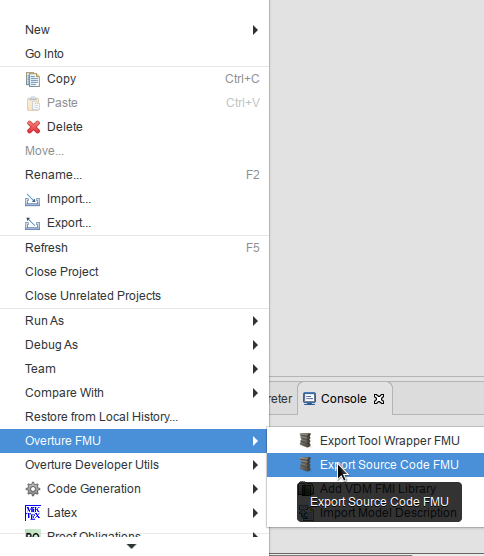
\includegraphics[width=3.5in]{figures/standaloneExportOverture.png}
\caption{Exporting a standalone FMU.}
\label{fig:standaloneexportoverture}
\end{figure}
%
%
%
%\clearpage